\chapter{绪论}

\section{研究背景及意义}

区块链(Blockchain)是一种按照时间顺序将数据区块以链条的方式组成的特定数据结构,被视为一个分布式的共享账本和数据库。它能够使用户无需相互信任与可信第三方的条件下完成可信的价值传输\cite{SurveyofEnterpriseBlockchains}。作为区块链2.0 的以太坊\footnotemark[1]\footnotetext[1]{\href{http://github.com/ethereum/wiki/wiki/White-Paper/}{以太坊白皮书}}重新将智能合约描述为图灵完备的、部署于区块链网络中合同条款代码。这意味着传统的合同条款可以进入实体计算机中,且在区块链网络去中心化、不可伪造、不可篡改的特性下严格执行。区块链推进了人与企业之间和线上与线下之间的全方面互联,其被成为下一代的新型生产关系。随着区块链的快速发展, 智能合约极大地丰富和扩展了区块链应用场景。它们为供应链、金融等传统领域带来重大变革, 已经快速渗入到人们生活的方方面面。

{\footnotesize
\begin{longtable}[h]{m{100pt}|m{50pt}|m{50pt}|m{50pt}|m{50pt}}
    \caption[主要公有云的BaaS平台]{主要公有云的BaaS平台} \label{major_BaaS_platforms} \\
        \hline  
        BaaS平台&Ethereum&Quorum&Corda&Fabric\\
        \hline
        AWS&Y&Y&Y&Y\\
        \hline
        Azure&Y&Y&Y&Y\\
        \hline
        IBM& & & &Y\\
        \hline
        阿里云区块链服务&Y& & &Y\\
        \hline
        腾讯云区块链服务TBaaS& & & &Y\\
        \hline
        华为云区块链服务BCS& & & &Y\\
        \hline
    \end{longtable}
}

与此同时, 云原生(Cloud native)作为一种基于云的基础之上的软件架构思想,以及基于云进行软件开发实践的一组方法论。因其弹性和分布式的优势成为当今流行的软件服务模式。云原生技术有利于各组织在公有云、私有云和混合云等新型动态环境中, 构建和运行可弹性扩展的应用, 借助平台的全面自动化能力, 跨多云构建微服务, 持续交付部署业务生产系统。区块链即服务(Blockchain as a Service, 简称BaaS)则是基于云原生技术体系的一种构建、管理、托管和运维区块链网络及其应用的云服务平台\cite{onik2019performance}。BaaS支持将任何企业级区块链实施到云环境,而无需任何IT专业知识。这大大降低了区块链技术的使用门槛, 是促使区块链技术更广泛、更深入地渗透到各个行业和企业的催化剂, 其市值预计从2018年的6.23亿美元猛增2023年的150亿美元\footnotemark[1]\footnotetext[1]{\href{https://www.reportbuyer.com/product/5486837/global-blockchain-as-a-service-market.html}{Global Blockchain-as-a-Service Market 2018-2022}}。其中, 云厂商提供了大多数的BaaS平台\cite{KuernetesbasedFabricChaincodeManagementAndHihgAvailabilityTechnology}, 如表\ref{major_BaaS_platforms}所示, 其底层区块链支撑技术大多数选择IBM开源的跨企业级联盟链Hyperledger Fabric, 这也是本文选择Hyperledger Fabric的原因。

% 挑战
然而, 当前BaaS平台的发展尤其是底层的区块链基础设施的建设依旧存在诸多挑战。

第一, 基础商业化应用工具并不完善\footnotemark[2]\footnotetext[2]{\href{http://www.caict.ac.cn/kxyj/qwfb/ztbg/202107/P020210726503897354430.pdf}{区块链基础设施研究报告(2021年)}}。虽然市场上存在多种可选择的BaaS平台解决方案, 但是这些BaaS平台由商业巨头把控, 行业马太效应明显\cite{KuernetesbasedFabricChaincodeManagementAndHihgAvailabilityTechnology}。BaaS平台的构建需要专业的区块链以及云原生的技术能力, 只有实力雄厚的云厂商进行BaaS平台的研发, 这些BaaS服务往往与云计算节点捆绑, 可用性限制通常会迫使其他企业为来自各种云提供商的基础设施即服务(Infrastructure as a Service, 简称IaaS)付费, 这导致了基于多云的网络\cite{DBLP:conf/coins/GerritsKKFV21}。

第二, 现阶段BaaS平台利用云能力对区块链基础设施赋能乏力。对于BaaS平台市场规模的不断膨胀, 需要找到解决当前区块链网络部署、备份、升级以及数据存储以及可扩展性的方法。区块链与云原生两种技术都相对不成熟, 但两者的集成可能会在技术方面产生新的复杂性\cite{onik2019performance}。当前BaaS平台仅提供了一种基于开源区块链平台的一键化自动部署管理方案, 未深入到区块链与云基础设施的底层。这并不是有效的云化方式, 浪费了云原生技术的潜力。区块链如何和云原生快速深度结合, 利用原生伸缩性、可移植性和高可用性价值来提供“高质量”的区块链服务,是当前仍然遗留的挑战。

\begin{figure}[h] %figure环境,h默认参数是可以浮动,不是固定在当前位置。如果要不浮动,你就可以使用大写float宏包的H参数,固定图片在当前位置,禁止浮动。
    \centering %使图片居中显示
    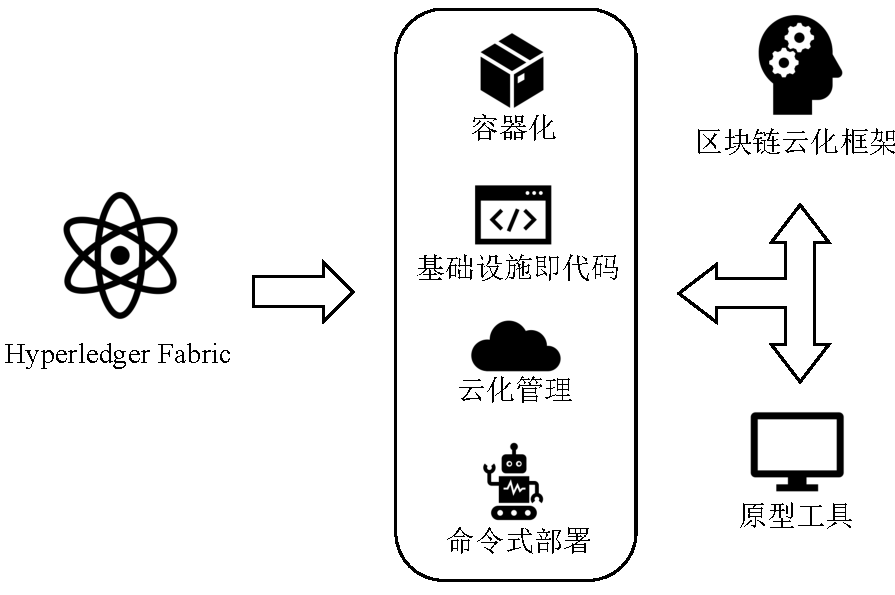
\includegraphics[width=0.7\textwidth]{FIGs/chapter1/framework_tool.pdf} %中括号中的参数是设置图片充满文档的大小,你也可以使用小数来缩小图片的尺寸。
    \caption{区块链云化框架及其原型工具} %caption是用来给图片加上图题的
    \label{framework_tool} %这是添加标签,方便在文章中引用图片。
\end{figure}%figure环境

% 意义、愿景
针对上述问题, 本文选择面向联盟链场景开源框架Hyperledger Fabric和Kubernetes针对BaaS平台的区块链基础设施提出了一种基于Hyperledger Fabric的区块链云化框架, 具体工作如图\ref{framework_tool}所示。该框架通过对Fabric网络中的Ca、Orderer、Peer组件进行抽象适配并利用Kubernetes Operator对其进行完整生命周期管理。本框架利用原生Kubernetes安全性、可扩展性等机制使用户通过专家提供的领域知识对Fabric网络获得类似云的自我管理。此外, 本文还实现了基于区块链云化框架的原型工具, 支持更简单、更原生的管理Fabric网络。

\section{区块链云化研究现状}

云原生背景下的区块链自诞生以来就受到了学术界与工业界的广泛关注。除了利用区块链的特性提升云的能力外\cite{DBLP:journals/comcom/XieZZWH21}\cite{DBLP:conf/smartcloud/SunWY20}\cite{8457813}, 研究人员也都期望自动化地构建出易于弹性扩展、高可用的区块链平台, 在区块链基础设施与云原生结合方面都开始了一定的探索。

% 学术
% 应用场景 BaaS平台往云上迁移
在学术研究方面, 研究人员在探究如何有效利用云平台来部署区块链平台。Gerrits等人\cite{DBLP:conf/coins/GerritsKKFV21}在Kubernetes中部署了分布式账本Hyperledger Sawtooth\footnotemark[1]\footnotetext[1]{\href{https://github.com/hyperledger/sawtooth-core}{Hyperledger Sawtooth github地址}}, 并运行了一个用例。他们旨在探讨该用例在真实场景云部署中的可行性和可扩展性。Liang等人\cite{liangeduchain}针对教育领域数据共享和信息欺骗的问题构建了一个高可用的教育联盟区块链平台, 并实现了基于Kubernetes的Fabric部署, 实现了将链码纳入Kubernetes环境管理的目标。

然而, Wan等人\cite{wan2018novel}指出当前主流的BaaS提供商通常采用API进行用户访问, 或者简单地将区块链应用迁移到云, 这会侵蚀不可信的机制并带来锁定风险。他们随后提出了一种新的服务范式来克服现有BaaS的局限性。基于Hyperledger的实施表明, 该范式可以缓解当前BaaS对区块链特征的侵蚀。在云原生底层基础设施方面研究人员关注与区块链结合的Kubernetes调度问题。才\cite{caili2018}在Kubernetes上面对PBFT和区块链的本身特性提出了静态调度和自适应算法。Shi等人\cite{9582270}为了解决云端现实PoS区块链工作负载的高效调度问题, 首次在云计算中设计和实现了基于Kubernetes的解决PoS区块链应用程序迁移成本的系统, 最大限度地减少了使用的Kubernetes工作节点数量以降低总体费用,而且还提出了一种高性能的Kubernetes调度方案HPKS以最大限度地利用工作节点进行在线pod管理。

% 工业界
相比于学术研究, 工业领域的探索更加注重自动化实践。Hyperledger Cello\footnotemark[1]\footnotetext[1]{\href{https://github.com/hyperledger/cello}{Hyperledger Cello github地址}}支持在多种底层基础设施上从头快速构建BaaS平台, 提供管理区块链网络的生命周期、自定义区块链网络配置等功能帮助人们以更高效的方式使用和管理区块链。Hyperledger Cello当前阶段重点关注在Docker安装, 对于Kubernetes支持方面的仍处在相对初级阶段, 配置项简单灵活性不足且老旧。Blockchain Automation Framework\footnotemark[2]\footnotetext[2]{\href{https://github.com/nikoturin/blockchain-automation-framework}{Blockchain Automation Framework github地址}}提供了一个自动化框架, 利用Ansible\footnotemark[2]\footnotetext[2]{\href{https://github.com/ansible/ansible}{Ansible github地址}}以及Helm\footnotemark[3]\footnotetext[3]{\href{https://github.com/helm/helm}{Helm github地址}}快速地、一致地将生产就绪的分布式账本技术(Distributed ledger technology, 简称DLT)平台部署到云基础设施。虽然, Blockchain Automation Framework提供了一个自动化框架将区块链平台部署于Kubernetes, 但本质上还是描述为一个需要希望远程主机执行命令的方案,或者一组IT程序运行的命令集合。这大大提升了自动化程度,但其远没有发挥Kubernetes的潜力。

% 总结
尽管学术界以及工业界目前已有一些关于区块链云化的探索与研究, 研究重点多为如何自动化地将区块链平台向云上迁移。总体来说目前的研究缺少构建支持云和区块链一体化的有效服务模型\cite{9582270}。

\section{本文主要研究工作}

% 本文主要的研究工作分为以下三个方面:

% 1.围绕领域驱动设计的战术建模过程展开了理论调研,
% 从《领域驱动设计:软件核心复杂性应对之道》\cite{DBLP:books/daglib/0013521}和
% 《实现领域驱动设计》\cite{vernon2013implementing}两本著作中抽取了八种战术建模模式及其重要特征。
% 具体地,针对八种战术建模模式,
% 设计了调查问卷,与工业界具有领域驱动设计实战经验的架构师和开发人员展开访谈;
% 根据访谈结果,通过多次焦点小组讨论,
% 对八种战术建模模式及其重要特征进行验证和完善,
% 克服了理论脱离实际的问题。
% 最终得出一套战术建模指南,该指南包括战术建模模式、模式属性、使用时机以及实现技术。


% 2.基于上述理论基础,通过UML profile机制扩展UML元类,实例化战术建模语言。
% 战术建模语言描述了战术模式的构造型、必要属性、关联关系以及重要约束。
% 以UML中元类为基础,更符合软件设计中面向对象(Object-Oriented)的思想,
% 也更易于软件从业者接受和学习。以该元模型为基础的建模语言,更关注战术建模,
% 包含最贴合实践的规则和约束,建模效率更高。

% 3.实现了一个战术建模支持工具,
% 该工具对建模过程中使用的战术模式进行约束与规范性校验,
% 对建模结果进行多种格式的转化与存储,
% 还包含生成框架项目代码包等扩展功能。
% 对战术建模支持工具进行了功能测试,并使用该工具进行了战术建模案例研究,
% 结果表明该工具支持开发人员快速理解各种战术模式的重要特征和规则约束,
% 降低了使用战术建模的学习成本;
% 可以对建模结果进行验证并提示开发人员进行修改,规范化建模过程;
% 还具有将建模结果转化为多种格式文件和框架项目代码的功能,使建模结果更具有通用性。


% 上述战术建模指南、战术建模语言以及战术建模支持工具共同组成了本文研究工作的战术建模支持方法及工具。

\section{本文组织结构}

本文组织结构如下:

第一章~绪论。介绍了本文的研究背景及意义、国内外研究现状、工业界的主要探索以及本文主要的研究工作;

第二章~理论与技术支持。介绍区块链尤其是Hyperledger Fabric的相关理论和概念; 同时介绍云原生的基本概念发展历程, 并对云原生基础设施Kubernetes进行了详细介绍;

第三章~基于Hyperledger Fabric的区块链云化框架。介绍区块链基础设施的现状及挑战, 基于这些现状区块链云化框架应当具有的设计原则, 并详细介绍了本文提出的基于Hyperledger Fabric的区块链云化框架。

第四章~原型工具设计与实现。;

第五章~框架检验与评估。;

第六章~总结与展望。

\section{本章小节}
